\documentclass[12pt]{article}
\usepackage{amsmath}
\usepackage{physics}
\usepackage{graphicx}
\usepackage[backend=biber, style=chem-acs]{biblatex}
\author{Patryk Kozlowski}
\title{Ch 121b Final Report}
\addbibresource{citations.bib}
\date{\today}
\begin{document}
\maketitle
\section{Introduction}
In the face of ambitious decarbonization goals, the Materials Genome Project attempts to expedite materials discovery for use in sustainability applications, e.g. photovoltaics or heterogeneous catalysis. Central in understanding the electronic structure of a material is its band structure, and more specifically its band gap. This helps to elucidate the conductivity properties of said material. One material of recent interest is the semiconductor gallium nitride, which crystallizes in the wurtzite structure.
\section{PySCF}
All computations were performed using the open-source PySCF package. \autocite{sun_recent_2020} There is a steep learning curve associated with learning this quantum chemistry package, but in the end, it is worth it because it allows one to efficiently tweak different parameters to the specific purpose. Additionally, the $G_0W_0$ code for periodic systems that was used \autocite{lei_gaussian-based_2022} is hosted on this platform.
\section{Methods}
Previous work shows that the hybrid functional B3PW91 outperforms the GGA of PBE and even self-consistent flavors of GW@PBE. \autocite{crowley_resolution_2016} However, in this work, the opposite was the case, likely because unoptimized structures were used for wurtzite gallium nitride as taken from the Materials Project. \autocite{noauthor_mp-804_nodate}
\subsubsection{Basis}
The Gaussian-type orbital basis sets (gth-szv and gth-dzvp) optimized for periodic calculations were used. Additionally, to minimize expense, a pseudopotential (gth-pade) was used.
\subsubsection{K-points}
Gamma point-centered k-point meshes of 1x1x1, 2x2x2, and 3x3x3 were used, for a total range of 1-27 k-points, Something like a 4x4x4 k-mesh (or larger) might be used for publication quality, but this was not that.
\subsection{DFT}
Standard approaches were used here. As expected, it was noticed qualitatively that calculations using the hybrid b3pw91 were more expensive than the respective GGA PBE ones.
\subsection{$G_0W_0$}
As previously mentioned, the periodic $G_0W_0$ code hosted on PySCF was used. The mean field object was a previous PBE calculation.
\subsubsection{Analytic Continuation}
Instead of performing an exact frequency integration, the code uses an analytic continuation scheme with an $O(N^4)$ scaling. This method avoids many of the poles on the real frequency axis, which can make solving the self-energy in the linearized quasiparticle iterative procedure (to mention one spectral quantity) tricky.
\subsection{Density Fitting}
Use of this code required a Gaussian density fitting routine of the  electron repulsion integrals from the mean field DFT object.
\section{Results}
\subsection{Sample Band Structure}
Although the primary focus of this work was in computing band gaps, band structures were also computed. Figure 1 shows one such example. The band gap (the Fermi energy between the maximum valence and minimum conduction bands indicated by the black and red lines, respectively, calculated at the Gamma point) is annotated.
\begin{figure}
\centering
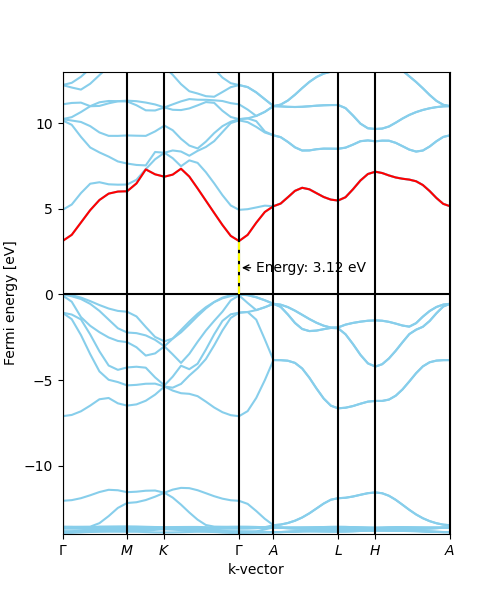
\includegraphics[width=0.72\textwidth]{pbe_dzvp_333_11-15.png}
\caption{Band structure of GaN computed with PBE functional at gth-dzvp basis and 3x3x3 k-point mesh.}
\end{figure}
\newpage

\subsection{Band Gaps}
The experimental benchmark at 1.6 K is 3.503 eV \autocite{madelung2004semiconductors}, as shown by the solid black line in the figures below. A finite size effect was observed with monotonic convergence towards a thermodynamic limit value as more k-points were sampled. The PBE functional gave better correspondence with experiment than b3pw91 across the board, regardless of the basis used or number of k-points sampled. Running $G_0W_0$ on the PBE mean field object at the larger gth-dzvp basis did not seem to give better correspondence with experiment than just regular KS@PBE in this work.
\subsubsection{Small Basis (gth-szv)}
\begin{figure}[h]
\centering
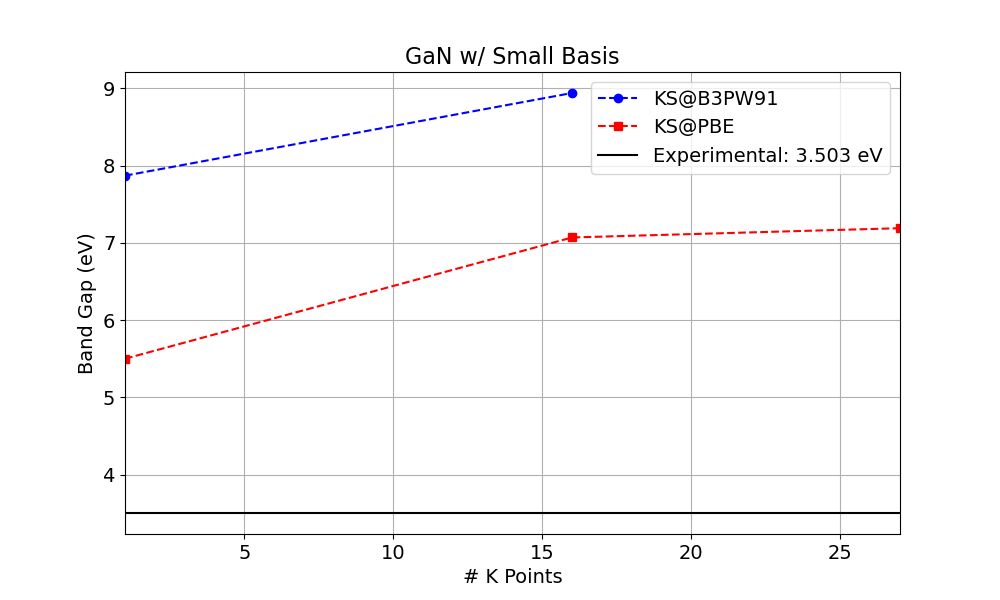
\includegraphics[width=\textwidth]{band_gaps_szv.png}
\caption{Band gaps computed with PBE and b3pw91 functionals at gth-szv basis}
\end{figure}
\subsubsection{Large Basis (gth-dzvp)}
\begin{figure}[h]
\centering
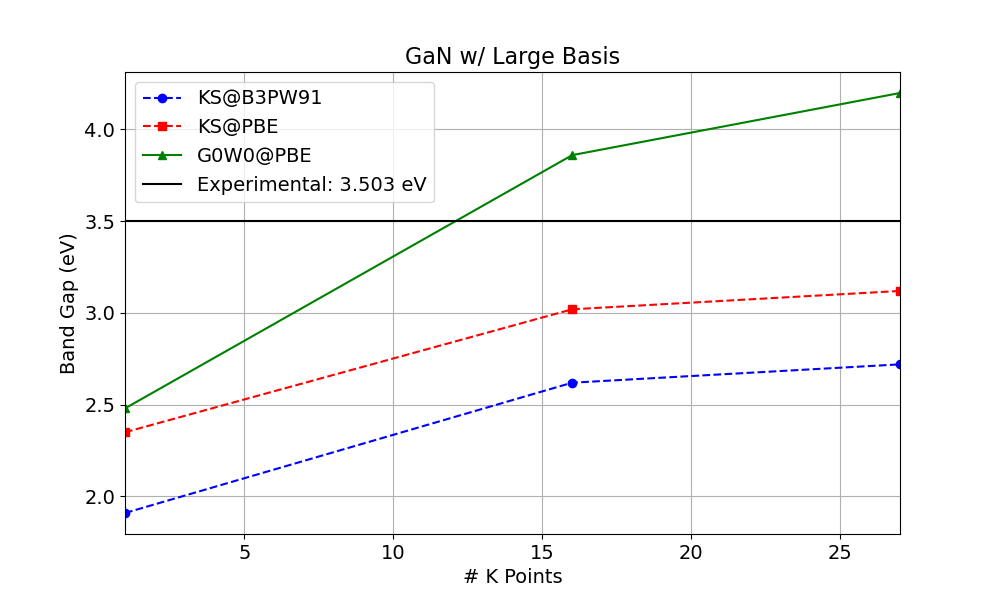
\includegraphics[width=\textwidth]{band_gaps_dzvp.png}
\caption{Band gaps computed with PBE, b3pw91, and $G_0W_0$@PBE at gth-dzvp basis}
\end{figure}
\newpage
\printbibliography
\end{document}